\cleardoublepage

\chapter{Implementación del protocolo blockchain}
Siguiendo las ideas planteadas en \ref{cap3} se ha realizado una implementación del protocolo blockchain, donde se han puesto en práctica los conceptos teóricos que se han tratado en este trabajo. 


Esta implementación funciona como un gestor de documentos donde se aprovecha el carácter inmutable de la estructura de cadena de bloques. Los participantes enviarán información en formato de cadena de caracteres, que bien puedan ser artículos, trabajos o cualquier otra clase de texto que desean almacenar. Esta información va debidamente firmada usando cierta clave privada, incluyéndose también la clave pública que permite verificar la firma. Utilizando el algoritmo de prueba de trabajo visto en \ref{chap3:pow} los nodos transformarán esta información en bloques de forma que se pueda tener un registro que sirva para probar que un trabajo fue verificado y existía desde un momento de tiempo concreto.


La implementación se encuentra disponible en el repositorio de Github \url{https://github.com/lglaria/TFG}

%Algunas ideas: (esto es opcional) cada participante debería disponer de dos hilos de proceso. Uno de ellos para interactuar con los otros nodos y otro para ejecutar el algoritmo de consenso. La idea es que en caso que alguien haya resuelto ese puzzle parar nuestro bucle del algoritmo de consenso.
%La solución anterior tiene menos sentido en nuestro caso, en el que el bucle del algoritmo de prueba de trabajo tiene un propósito. Sin embargo, en otro entorno sí que podría ser útil esta implementación. Se podrían implementar ambas,
\section{Características de la implementación}
El algoritmo de consenso elegido ha sido el de prueba de trabajo, combinado con la elección de la cadena de bloques más larga en caso de tener varias alternativas disponibles.

Los bloques de la cadena son arrays de Python y almacenan (en ese orden):
\begin{itemize}
\item El valor hash del bloque anterior en formato hexadecimal. Excepto para el bloque inicial al que se le asigna por defecto el valor cero en este campo.
\item La información que se desea guardar así como la firma y la clave pública de quien ha enviado (o validado) este texto. En el bloque inicial se pone el valor cero.
\item Una marca temporal, se ha usado el sistema UNIX timestamp
\item Un índice incremental. Empieza en cero en el bloque inicial.  
\item El nonce del bloque. Cadena de 32 bits a partir del algoritmo de prueba de trabajo. Este algoritmo ha sido implementado de forma similar a lo visto en \ref{chap3:pow}
\end{itemize}

\lstset{language=Python}
\lstset{frame=lines}
\lstset{caption={Algoritmo de prueba de trabajo}}
\lstset{label={lst:code_direct}}
\lstset{basicstyle=\footnotesize}
\begin{lstlisting}[frame=single]
def pow(self,bloque): #algoritmo de prueba de trabajo
  bloque_str = ''.join(str(e) for e in bloque)
  while True:
    var = format(random.getrandbits(32), '08b') #buscamos nonces de 32 bits
    hash_value = sha256((bloque_str+str(var)).encode('utf-8')).hexdigest()
    if hash_value[:self.longitud_nonce] == '0'*self.longitud_nonce:
      break
  bloque.append(var)
  return bloque
\end{lstlisting}


\section{Aspectos técnicos.}
En esta implementación se ha utilizado el lenguaje de programación Python. Para el proceso de firma basado en el algoritmo ECDSA se ha recurrido la librería \textit{fastecdsa} \citep{fastecdsa}. En concreto, se ha usado la curva elíptica p-256 del Instituto Nacional de Estándares y Tecnología (NIST) dependiente del Departamento de Comercio de los Estados Unidos. El algoritmo de firma basado en la curva anterior cumple con los requisitos de seguridad mencionados en el capítulo \ref{cap1}.

En la implementación del algoritmo de prueba de trabajo se ha utilizado la función hash SHA-256 que ya fue mencionada en la sección \ref{chap3:pow}. Esta función, ampliamente utilizada en diversas implementaciones del blockchain, se ha obtenido a través de la librería \textit{hashlib} \citep{hashlib}. Los nodos calculan el nonce generando valores aleatorios de 32 bits. Por defecto se ha puesto una dificultad fija, pero este valor puede ser modificado y calculado a partir de una función tal y como ocurre en el Bitcoin. En el cálculo del nonce no se modifica el timestamp.


Se almacena en cada nodo el conjunto de las operaciones y no la raiz Merkle del arbol resultante. Esto puede igualmente ser modificado.

Por último, la red p2p sobre la que funciona el protocolo se ha construido usando la librería \textit{multiprocessing} \citep{multiprocessing}. Con esta librería se solucionan los problemas de concurrencia que podrían aparecer al mantener activos al mismo tiempo dos procesos que trabajan sobre la misma estructura de datos: uno para recibir los mensajes que le llegan a un nodo y otro para ejecutar el algoritmo de consenso, actualizar la cadena y transmitir información.


Esta implementación puede igualmente ser aplicada en un entorno real basado por ejemplo en bases de datos de tipo SQL. En este supuesto se podria utilizar el valor hash de cada bloque como referencia de las entradas de la tabla.


\section{Seguridad de la implementación y posibles mejoras.}
Queda por hacer un análisis similar al de la sección \ref{cap3:seguridad} para esta implementación en concreto, ignorando los supuestos de privacidad que carecen de sentido en este caso. La fortaleza del algoritmo de cifrado y de la función hash dependen de las librerías elegidas para usar estos métodos y de acuerdo con la documentación no tienen problemas de seguridad conocidos.
Hay que ver por tanto si el consenso que busca alcanzar este implementación es vulnerable a algún tipo de ataque. 


Un posible agresor podría intentar realizar dos tipos de acciones que alteren el consenso:

\begin{enumerate}
\item Incluir en la cadena información incorrecta.  
\item Modificar la cadena para incluir nuevos bloques en determinada posición (distinta de la última) o modificar bloques existentes.
\end{enumerate}

Dado que este protocolo no dispone de un mecanismo para distinguir cuando un texto es correcto o no, y como en general tales mecanismos automáticos resultan difíciles de modelar una posible solución es hacer que esta implementación funcione como blockchain de consorcio o privado. Esto tiene sentido pues en una situación real quienes se encargan de verificar que un documento o trabajo cumple con ciertos criterios son exclusivamente las personas autorizadas a ello. De esta forma, aunque se pueda incluir información incorrecta al final de la cadena esto será responsabilidad de quien la haya firmado. La lista de claves públicas autorizadas a realizar validaciones se podría añadir como un campo más en la cadena de bloque o mantener una estructura de datos alternativa donde se almacene esta lista. Además de verificar que la firma se corresponde con la clave pública habría también que comprobar también que esta clave está autorizada a verificar documentos.

El segundo tipo de ataque como se vio en el capítulo \ref{cap3} depende de la dificultad de la función hash y de la longitud de la cadena. Un atacante que quiera modificar algún bloque sabemos debería rehacer toda la cadena, pues los valores hash que señalan al bloque anterior y por tanto el nonce del algoritmo de prueba de trabajo habría que volverlos a calcular. Pero ahora no dependemos solamente de la dificultad de esta operación (que por sí sola garantizaría la seguridad) sino que se puede aprovechar el hecho de disponer de un conjunto definido de claves públicas autorizadas a validar. Si además de firmar el texto hacemos que haya que firmar el valor hash del bloque anterior, un posible atacante debería disponer de alguna clave privada y además de eso la cadena falsa que genere se caracterizará por incluir a partir de la posición donde ha realizado la modificación una única firma, lo que hace muy fácil identificar esta clase de ataques.


\section{Cálculos sobre el algoritmo de prueba de trabajo}
Cuando se explicó el funcionamiento del algoritmo de prueba de trabajo se hizo referencia a la relación entre la longitud del puzzle (la condición que se le impone al valor hash que se considere válido) y al tiempo de procesamiento necesario para obtener este valor. Dado que ahora se dispone de una implementación de este algoritmo es posible comprobar este hecho en la práctica.

Se incluye una tabla con los tiempos medios que se tardado en obtener el nonce según la dificultad para ciertas cadenas generadas de forma aleatoria.
\begin{table}[htb]
\centering
\begin{tabular}{|l|l|l|}

\hline
Dificultad (ceros del hash)  & Tiempo medio (segundos) & Número de iteraciones \\
\hline \hline
1 & 9.87052917e-05 & 100\\ \hline
2 & 1.49291515e-03 & 100\\ \hline
3 & 3.24990416e-02 & 100\\ \hline
4 & 4.12933254e-01 & 100\\ \hline
5 & 6.35731197e+00 & 100\\ \hline
6 & 9.97811596e+01 & 10 \\ \hline
\end{tabular}
\caption{Resultados algoritmo prueba de trabajo.}
\label{tabla:anchofijo}
\end{table}

Aunque estos valores dependen de la máquina en la que se efectúen los cálculos, y en este caso por limitaciones técnicas no ha sido posible realizar más comprobaciones, puede apreciarse que hay relación directa entre la longitud de la cadena pedida como solución del problema y el tiempo necesario para encontrarla.

\begin{figure}[H]
%\centering
  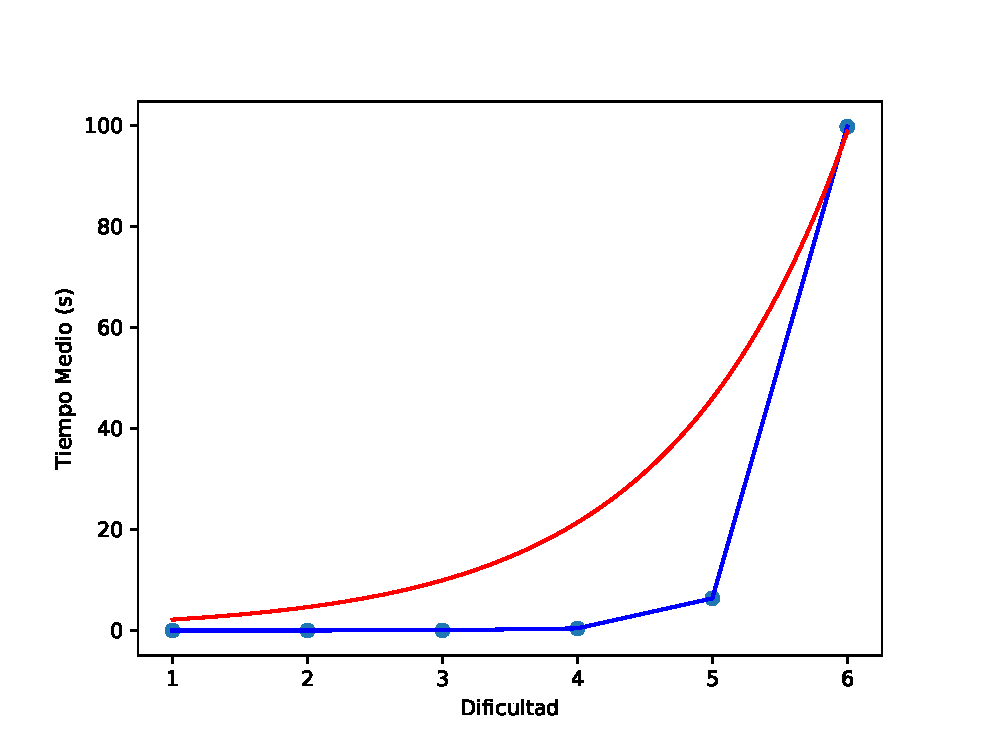
\includegraphics[width=12cm]{figures/resultados_pow.eps}
  \caption{Comparación entre los resultados y la función $y = 2^x$}
  \label{fig:resultados}
\end{figure}
En la figura \ref{fig:resultados} se aprecia que los resultados obtenidos tienen un comportamiento similar a la función $y(x) = 2^x$. Aunque esto no puede considerarse como una aproximación buena del algoritmo de prueba de trabajo con la función hash SHA-256, pues ni el tamaño de la muestra es lo suficientemente grande, ni se han hecho comprobaciones para dificultades superiores a 6, sí es un indicador de que este comportamiento es cuasi-exponencial.
%Implementaremos el algoritmo visto en \ref{chap3:pow}
%Uno de los problemas del algoritmo de prueba de trabajo del Bitcoin es que todo el esfuerzo en términos de procesamiento que se usa para resolver el puzzle es en esencia inútil (no es verdaderamente inútil, pues cumple la función para la que está diseñado...). Esto está detrás de las graves implicaciones medioambientales del Bitcoin y de otras populares criptomonedas (poner referencia y datos sobre el consumo energético). Lo que proponemos es utilizar los cálculos con las funciones hash en el algoritmo de prueba de trabajo para buscar colisiones en la función SHA-256, tal como se definieron en \ref{hash}